\section{Final Assignment}

For the final assignment, I am managing a database using SQL and the ESP32.
I chose for this assignment because of the likelihood that the ESP32 has to interact with a database for the final product.
The goal of this assignment is to make the ESP32 able to log certain events, which will be stored into a database.
The event that will be logged is the pressing down of a push button.
The ESP32 will not communicate directly with the database; instead, it communicates with the database via a web server.
This is removes the need for the ESP32 to run a heavy SQL client and instead a much simpler HTTP client can be used.

\subsection{Demonstration Setup}

\begin{figure}[htbp]
    \centering
    \begin{circuitikz}
        \ctikzset{multipoles/dipchip/pin spacing=0.2}
        \ctikzset{resistor=european}
        \draw (0,0) node[dipchip,
            num pins=30,
            hide numbers,
            external pins width=0.1,
            external pad fraction=3](C){ESP32};

            \draw (C.pin 15) -- ++(-0.5,0) -- ++(0,-0.5) -- ++(3,0) -- ++(0,5) -- ++(-3,0) coordinate (P1);
            \draw (C.pin 14) -- ++(-0.5,0) to[R] ++(-2.0,0) -- ++(0,1.5) to[push button] ++(0,1) coordinate (P2) -- (P2|-P1) -- (P1);
            \draw (C.pin 11) -- ++(-2.5,0);

            \node [right,font=\tiny]
            at (C.bpin 11) {GPIO27};

            \node [right,font=\tiny]
            at (C.bpin 14) {GND};

            \node [right, font=\tiny]
            at (C.bpin 15) {5V};
    \end{circuitikz}
\end{figure}

\noindent
I used the circuit above to connect the push button to the ESP32.
The locations of the pins may differ depending on which version of the ESP32 is being used.
As for setting up the software, the client is flashed onto the ESP32 and the web server and the database are hosted a Raspberry Pi.
I configured port forwarding on my home network so that the ESP32 can communicate with the web server from other networks.

\subsection{Development Environment and Tooling}

For programming the ESP32, I decided on using the ESP-IDF.
I have used the \code{idf.py} command-line tool for building and flashing the project.
For configuring the web server and database I used OpenSSH, to establish a SSH connection.
I wrote the code using the Vim text editor and used Git for version control.

\subsection{Used Software Libraries}

For the client, I have used libraries that come with ESP-IDF.
These libraries allowed me among other things to establish a \gls{wifi} connection and perform \gls{http} requests.
For the server, I used Go's standard library packages for working with \gls{http} and SQL.
Go's standard library package \href{https://pkg.go.dev/database/sql}{database/sql} does not work with MySQL out of the box.
I had to use another package that enables MySQL support for Go's \href{https://pkg.go.dev/database/sql}{database/sql} standard library package.
This package contains a Go driver for MySQL and can be found at: \url{https://github.com/go-sql-driver/mysql}.

\subsection{Software Architecture}

The software consists of three major components: a \gls{http} client, a \gls{http} server, and a relational database.
The ESP32 is communicating with the web server and the web server communicates with the database.
The client makes \gls{http} requests to the server, after which the server will query the database based on the request being made.
There are two types of request that can be made: one for creating new users and another one for logging events.
I have put the \gls{erd} of the database below.
The database consists of two tables: one for storing patient data and another one for holding logs.

\begin{center}
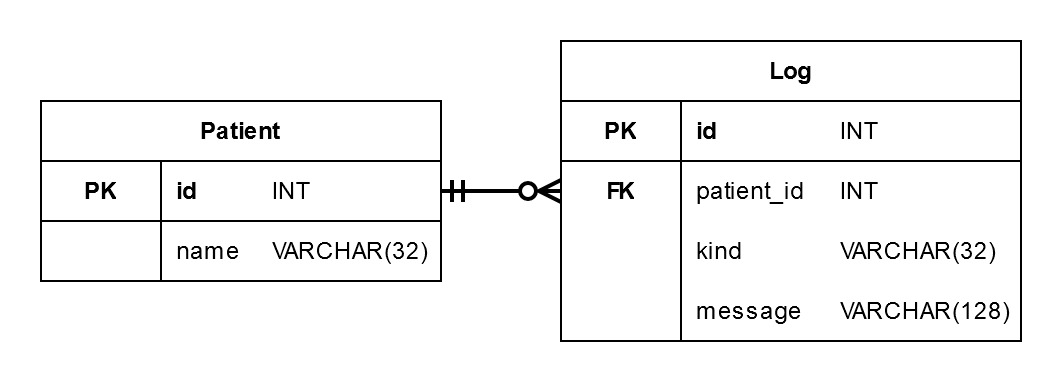
\includegraphics[width=\textwidth]{images/erd}
\end{center}

%Of these components, the  server and the database are hosted a Raspberry Pi, while the  client runs on an ESP32.
%The \gls{http} client communicates with the \gls{http} server, which in turn communicates with the database.
%The ESP32 is interacting with the database via a web server as hosting a SQL client would be a very intensive task for a microcontroller.

\subsection{Results}

At first instance, I wanted to query the database directly from the ESP32.
However, I soon found out that this was a non-trivial task.
This would require the ESP32 to run a SQL client.
While I found online resources on how to do this
I decided instead to use a HTTP server.


I came a challenge for how to designing the software architecture.
I did not experience any problems when working on this assignment.
However, I did come accross some challenges for the design.
At first instance I thought 
A SQL client is 

\subsection{Accountability}

I have done this assignment by myself.

\clearpage

